\documentclass[10pt,twocolumn]{article}

\usepackage[margin=0.75in]{geometry}
\usepackage{times}
\usepackage{microtype}
\usepackage{graphicx}
\usepackage{booktabs}
\usepackage{amsmath}
\usepackage{enumitem}
\usepackage[numbers,sort&compress]{natbib}
\usepackage[hidelinks]{hyperref}
\usepackage{tcolorbox}
\usepackage{xcolor}
\usepackage{tikz}
\usepackage{tabularx}
\usepackage{fancyvrb}
\urlstyle{same}
\renewcommand{\ttdefault}{cmtt}

% ── Flag macros (TikZ inline) ─────────────────────────────────────────────────
\newcommand{\flagCH}{%
\tikz[baseline=-0.55ex, x=1em, y=1em]{
  \fill[red!85!black] (0,0) rectangle (1.15,0.8);
  \fill[white] (0.48,0.14) rectangle (0.67,0.66);
  \fill[white] (0.25,0.305) rectangle (0.90,0.495);
}}
\newcommand{\flagBE}{%
\tikz[baseline=-0.55ex, x=1em, y=1em]{
  \fill[black] (0,0) rectangle (0.38,0.8);
  \fill[yellow!85!orange] (0.38,0) rectangle (0.76,0.8);
  \fill[red!80!black] (0.76,0) rectangle (1.15,0.8);
}}
\newcommand{\flagBA}{%
\tikz[baseline=-0.55ex, x=1em, y=1em]{
  \fill[blue!70!black] (0,0) rectangle (1.15,0.8);
  \fill[yellow!90!orange] (0.43,0.8) -- (1.15,0.8) -- (1.15,0.0) -- cycle;
  \foreach \x/\y in {0.43/0.72,0.52/0.62,0.61/0.52,0.70/0.42,0.79/0.32,0.88/0.22,0.97/0.12}{
    \node[white, scale=0.22] at (\x,\y) {$\star$};
  }
}}
\newcommand{\flagGB}{%
\tikz[baseline=-0.55ex, x=1em, y=1em]{
  \fill[blue!70!black] (0,0) rectangle (1.15,0.8);
  \draw[white, line width=0.19em] (0,0) -- (1.15,0.8);
  \draw[white, line width=0.19em] (0,0.8) -- (1.15,0);
  \draw[red!85!black, line width=0.09em] (0,0) -- (1.15,0.8);
  \draw[red!85!black, line width=0.09em] (0,0.8) -- (1.15,0);
  \fill[white] (0,0.29) rectangle (1.15,0.51);
  \fill[white] (0.46,0) rectangle (0.69,0.8);
  \fill[red!85!black] (0,0.34) rectangle (1.15,0.46);
  \fill[red!85!black] (0.515,0) rectangle (0.635,0.8);
}}

\setlength{\columnsep}{0.25in}
\setlength{\parindent}{1em}
\setlength{\parskip}{0pt}
\raggedbottom

\title{\textbf{Cross-Constituency Aggregation for Community Notes}}

% Three authors sharing one affiliation. Stacking them with \and overflows the
% narrow first column in this twocolumn layout, so the names sit on one line
% above a single shared affiliation.
\author{
Emrecan Ulu, Jingyao Shi, Carina I. Hausladen\\
University of Konstanz\\[2pt]
% Code and data pointer, on page one under the names. The title block spans both
% columns, so the full repository URL fits on one line here.
{\small\url{https://github.com/vulonviing/cross-constituency-aggregation-community-notes}}
}

\date{}

\begin{document}

\maketitle

\begin{abstract}
Community Notes is X's crowd-based fact-checking system: contributors write
contextual notes, other contributors rate them, and a bridging algorithm decides
which notes become visible. The algorithm is designed to avoid simple majority
capture by estimating note quality separately from ideological alignment, so a
note should gain support across disagreement rather than only within one side
\citep{wojcik2022birdwatch,xcommunitynotes2026ranking}. Because the system
works through sparse and unequal participation, display decisions can depend
heavily on a relatively small active core, and many notes remain in Needs More
Ratings when the algorithm does not find enough diverse support
\citep{goyal2026qsmf,razuvayevskaya2025timeliness}. We argue that this is not
only a data-sparsity problem but an aggregation problem: Community Notes treats
cross-group agreement indirectly, through a fitted model, rather than as an
explicit decision rule over constituencies.

We take inspiration from political science and social choice, where systems
such as Switzerland's double-majority referendum rule treat cross-group support
as part of a decision's legitimacy. A note should not become visible because
one active group overwhelms the rest; it should become visible when each
relevant constituency has a real chance to support it. We operationalize this
as cross-constituency aggregation, recovering behavioral constituencies from
co-rating patterns among 200,000 active raters, compute each note's approval
rate inside each constituency, and combine those rates with a geometric mean
under a minimum-coverage rule. In a 100,000-note analytical slice, Community
Notes displays 6,832 of 44,722 representative-picked notes (15\%). Our rule
identifies a 13,655-note rescue pool, raising potential visibility to 20,405
notes (46\%) before validation. A second-stage validation screen judges 8,558
candidates, 63\% of the pool, to be sourced and rescue-worthy. These results suggest
that useful notes can remain hidden when cross-group support is modeled only
indirectly.
\end{abstract}

\section{Introduction}

Community Notes is X's crowdsourced fact-checking system. When a post may need
context, contributors write a short note and others rate whether it is helpful;
if a note gathers enough support, it is shown under the post. Rather than relying
on professional fact-checkers or automated classifiers, the platform asks a crowd
to decide which context becomes visible
\citep{wojcik2022birdwatch,xcommunitynotes2026ranking}.

The key innovation is a bridging algorithm. A simple majority vote would be easy
for one political side or one active group to capture, so X scores notes with a
matrix factorization over the sparse note-rater matrix
(Section~\ref{sec:how_cn_works}), crediting a note only for support that
viewpoint compatibility cannot explain. That factorization is the core ranking
layer rather than the full pipeline, which adds agreement safeguards,
engagement and independence checks, and a November 2025 geometric-mean pilot
\citep{xcommunitynotes2026ranking}.

The design is powerful but incomplete. Note helpfulness is still estimated from
sparse, uneven ratings, which recent work shows is sensitive to noisy,
strategic, and hyperactive raters \citep{goyal2026qsmf,nudo2026hyperactive},
and participation is steeply unequal (Section~\ref{sec:the_gap}), so a formally
open crowd can still turn on a small, active core. More basically, the model
keeps group support inside a fitted estimate: it never forms a quantity such as
``approval inside constituency A'' versus ``approval inside constituency B,''
so cross-group acceptance is present only indirectly.

We start from a different premise. Instead of estimating which raters are more
reliable as individuals, we treat recovered behavioral constituencies as
legitimate parts of the crowd and ask whether a note is acceptable across them.
This turns Community Notes from a prediction problem into a crowd-agreement
problem: the platform is deciding, in the name of ``the community,'' whether a
note should attach to a public post. The question follows directly:

\begin{quote}
When ratings come from behaviorally distinct constituencies, which aggregation
rule should decide whether a Community Note becomes visible?
\end{quote}

The inspiration is political science and social choice rather than another
rater-quality model. Divided societies use power sharing, double majorities,
parallel consent, or veto-like rules so that collective decisions depend on
support traveling across groups, not only on the strongest or most active side
\citep{lijphart1977democracy,mcgarryoleary2009,horowitz1991makingmoderation,reilly2002electoral},
and social-choice theory gives a formal version of the same idea
\citep{peters2019proportionality,qiu2025representative}. We borrow this logic in
a limited way. Community Notes is not a state, and displaying a note is not
passing a law. Still, both settings face the same aggregation problem under
disagreement.

This logic yields four criteria for the display decision:
\begin{itemize}[leftmargin=*,itemsep=2pt,topsep=3pt]
    \item \textbf{P1 (Presence).} Every constituency must be present in the
    decision.
    \item \textbf{P2 (Non-compensation).} One constituency's rejection should
    not be fully compensated by another's enthusiasm.
    \item \textbf{P3 (Symmetry).} Constituencies should enter the rule
    symmetrically, so that no group is privileged by default.
    \item \textbf{P4 (Behavioral recovery).} Since no constituencies are given
    in advance, they must be recovered from observed rating behavior rather than
    assigned from outside labels such as party, country, or ideology.
\end{itemize}

We operationalize these criteria as cross-constituency aggregation. Using the
active 200k Representative pipeline, we cluster active raters from co-rating
behavior, reassign them into two main behavioral constituencies, compute each
note's approval rate inside each constituency, and combine these rates with a
geometric mean under a minimum-coverage requirement. The geometric mean creates a
soft veto: if either constituency strongly rejects a note, the final score falls,
even if the other constituency is highly supportive. We then use this score to
identify hidden Community Notes that deserve a second look, and we validate those
candidates separately for sourcing, content type, and rescue-worthiness.

On a 100,000-note slice of the live sample, the rule surfaces a 13,655-note
rescue pool the platform currently leaves hidden, of which a second-stage screen
keeps 8,558 as sourced and rescue-worthy. Community Notes therefore has an
aggregation problem as well as a rating problem: useful public-interest notes
can remain hidden when cross-group support is modeled only indirectly.

\section{How Community Notes Works}
\label{sec:how_cn_works}

X's Community Notes pipeline does not determine note visibility through a simple majority vote. Instead, it uses a matrix factorization algorithm designed to find consensus across polarized groups, a concept the platform calls ``bridging'' \cite{wojcik2022birdwatch}. The system decomposes the predicted rating $\hat{r}_{un}$ given by a rater $u$ to a note $n$ using the following formula:

\begin{equation}
    \hat{r}_{un} = \mu + i_u + i_n + f_u \cdot f_n
    \label{eq:cn-model}
\end{equation}

This equation breaks a rating down into four distinct components to isolate the note's baseline helpfulness:
\begin{itemize}
    \item $\mu$ \textbf{(Global Intercept):} The baseline rating tendency across the entire platform.
    \item $i_u$ \textbf{(Rater Intercept):} A measure of whether a rater is generally generous or strict when evaluating notes.
    \item $i_n$ \textbf{(Note Intercept):} \textbf{The target metric.} This represents the note's pure helpfulness score, stripped of ideological alignment and rater bias.
    \item $f_u \cdot f_n$ \textbf{(Viewpoint Match):} The dot product of the rater's latent factor ($f_u$) and the note's latent factor ($f_n$). It captures how well the note aligns with the rater's political or behavioral ideology.
\end{itemize}

\subsection*{A Critique of Matrix Normalization: Profiling Over Consensus}
The terms $i_u$ and $f_u \cdot f_n$ do not measure ``bad faith''; they act as normalization tools. But by relying on them, the core action of Community Notes shifts from evaluating the \textit{content} of a note to estimating the \textit{intent} of the user. Simulation studies of the open-source algorithm make this concrete: a coordinated minority of just 5--20\% of biased raters can suppress genuinely helpful notes outright \citep{truong2025vulnerable}. Observers have questioned the system's narrow reliance on cross-group consensus \citep{jude2025narrow}; our concern is more specific: the model identifies that consensus by first estimating users' rating tendencies and viewpoint alignment, grounding its judgment of the note in inferences about the users who rated it.

To isolate note quality ($i_n$), the algorithm treats rater tendencies and viewpoint compatibility as structural noise (Figure~\ref{fig:rater-dominance-schematic}), and in doing so profiles users and reads their intentions: is this user voting on objective truth, or cheering for their side? The result is an implicit hierarchy of raters, on the assumption that weighting ``high-quality,'' unbiased evaluators is the most effective way to govern visibility.

Recent literature highlights the fatal flaw in this intent-reading framework. \citet{goyal2026qsmf} and \citet{nudo2026hyperactive} demonstrate that such quality-estimation structures are highly vulnerable to manipulation by strategic voters and ``hyperactive minorities.'' Inferring rater quality from a sparse matrix, the model comes to lean on whoever rates most often: if a hyperactive minority dominates the rating record, their voting patterns dictate the latent space, and an algorithm hunting for ``quality raters'' inside such a lopsided pool amplifies that core rather than capturing community consensus.

\begin{figure*}[t]
  \centering
  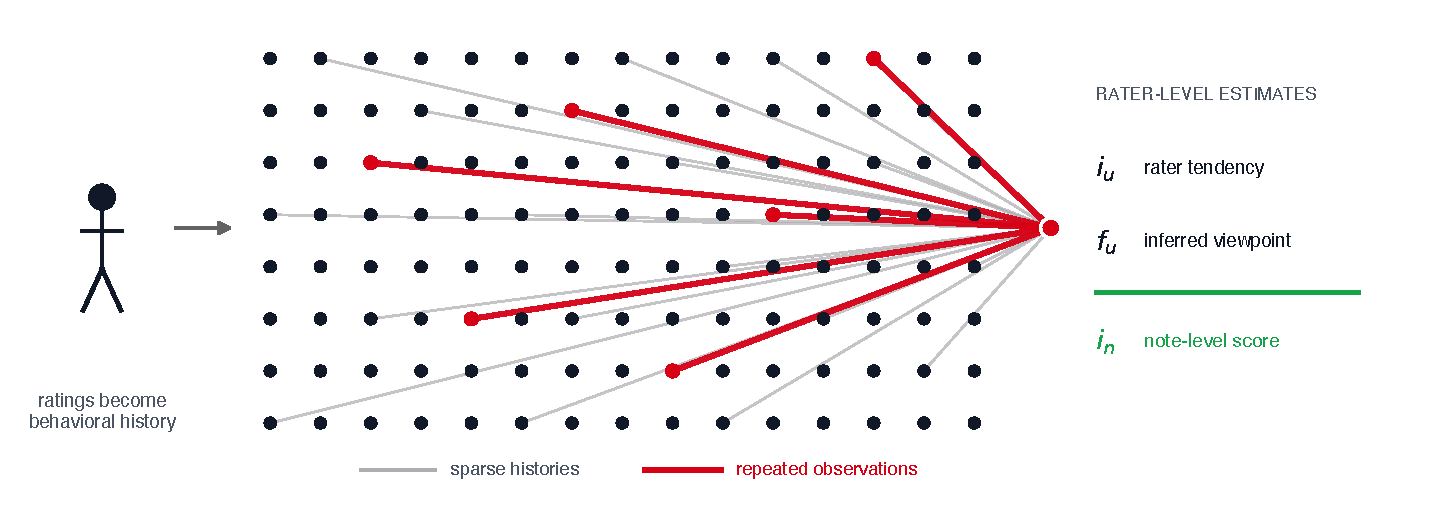
\includegraphics[width=0.93\textwidth]{../figures/script_figures/fig1-rater-dominance.pdf}
  \caption{Repeated participation gives a small set of highly active raters more
  leverage over the latent space fitted by matrix factorization. The model does
  not assign these users an explicit vote weight. Instead, their longer rating
  histories contribute more observations to the estimates of rater tendency
  ($i_u$) and viewpoint ($f_u$), which the pipeline uses before isolating the
  note-level score ($i_n$). The diagram is schematic and not drawn to scale.}
  \label{fig:rater-dominance-schematic}
\end{figure*}

\subsection*{The Algorithm in Practice: A Conceptual Map}
Two of the algorithm's cases are easy to state. A partisan rater who approves a
note flattering their own side earns it nothing: the viewpoint match
$f_u \cdot f_n$ already predicted that vote, so $i_n$ stays flat and the note
stays hidden \cite{wojcik2022birdwatch}. The reverse case is where the model
earns its keep. When two raters at opposite poles independently mark the same
note ``Helpful,'' viewpoint alignment can explain nothing, the surplus has
nowhere to land but $i_n$, and the note surfaces as carrying something true
enough to cross partisan lines \cite{buterin2023what}.

The third case is corrosive rather than additive. Both stories above assume the
algorithm holds an honest map of where each rater sits in the latent space. It
does not start with one; it draws the map from the rating record, and a few
hands draw most of it. Think of a class graded on participation where the
teacher keeps asking ``what does the class think?'' but the same handful of
students answer every session, until their voices become the teacher's idea of
the whole room. Community Notes inherits this distortion: a hyperactive,
politically polarized minority supplies most ratings, so their behavior fixes
where the axis of ``viewpoint'' lies and which votes look ``surprising''
\cite{nudo2026hyperactive}. Once a narrow crowd has drawn the map, the
``enemies'' whose handshake looked so convincing may be two wings of the same
faction, and the bridge the model celebrates spans a gap most users were never
placed on.

\section{The Gap in Community Notes}
\label{sec:the_gap}

\subsection*{The Platform's Defense: Bridging}
X officially defends its algorithm using a ``bridging'' analogy \cite{xcommunitynotes2026ranking}: a note supported only from one side of the polarization axis stays hidden, and visibility requires positive ratings from raters the model places at opposite ends of the latent viewpoint dimension. Platform engineers argue this prevents majority tyranny and resists coordinated manipulation by any single faction.

\subsection*{Why the Defense Does Not Hold}
The bridging claim rests on a prior step that undermines it. Before any cross-group comparison can take place, the formula of Section~\ref{sec:how_cn_works} must situate every rater in a two-dimensional space of inferred identity. Two terms do this work. $i_u$ collapses each rater to a leniency or strictness tendency, from which a rater who is critical because they apply high standards cannot be distinguished from one who systematically opposes certain content. The viewpoint term $f_u \cdot f_n$ goes further, pinning each rater to a coordinate on an axis the model derives entirely from co-voting patterns; a ``Helpful'' rating counts as cross-group signal only when the model could not have predicted it from that coordinate. Bridging, operationally, means ``this approval was surprising given where we placed this rater,'' not ``two independent communities both endorsed this note.''

The resulting action is intent inference rather than content evaluation. The algorithm asks not \textit{what} a note says, but \textit{who} tends to approve notes like this. Sparse, unequal participation makes the inference less reliable still: when a small hyperactive minority supplies most of the votes that fix the latent axis, the coordinate system reflects their behavioral patterns, not the broader community's.

\subsection*{Evidence from Our Own Pipeline}

\begin{table}[t]
\centering
\small
\resizebox{\columnwidth}{!}{%
\begin{tabular}{lcrrrrrl}
\toprule
& & \multicolumn{3}{c}{Initial spectral partition} & \multicolumn{2}{c}{After Method B} & \\
\cmidrule(lr){3-5}\cmidrule(lr){6-7}
Scale & $k$ & ARI & Pearson & Discrim. & Pearson & Discrim. & Hyperactive outlier \\
\midrule
60k  & 2 & 0.989 & $-$0.69 & 86\% & --- & --- & absorbed (none) \\
150k & 3 & 0.977 & $-$0.65 & 83\% & $-$0.644 & 82.9\% & 62 users ($\sim$7$\times$) \\
200k\textsuperscript{$\dagger$} & 3 & 0.971 & $-$0.62 & 82\% & $-$0.620 & 81.4\% & 64 users ($\sim$11$\times$) \\
210k & 3 & 0.969 & $-$0.62 & 81\% & $-$0.617 & 81.2\% & 66 users ($\sim$12$\times$) \\
240k & 4 & 0.955 & $-$0.60 & 80\% & $-$0.596 & 80.0\% & 60 + 1{,}431 ($\sim$25$\times$) \\
250k & 2 & 0.997\textsuperscript{$\ddagger$} & --- & --- & --- & --- & degenerate: 249{,}933~/~67 \\
\bottomrule
\end{tabular}}
\caption{Clustering stability across scale. The initial columns report the partition the algorithm selects on the raw co-rating graph, before reassignment: $k$ is the cluster count chosen by bootstrap stability, ARI the mean bootstrap ARI at that $k$. Above 60k this partition still holds the hyperactive raters apart. The Method B columns report the final two-camp partition after vote-profile reassignment, measured on notes with at least ten raters per camp. Pearson correlates the two main camps' note-level approval rates; Discrim.\ is the share of notes whose between-camp gap exceeds 0.3. The last column gives the separated sub-population and its median vote count relative to the main camps; at 60k nothing falls below the outlier threshold, so reassignment does not apply.}
\label{tab:scaleup}
\begin{flushleft}
\footnotesize
\textsuperscript{$\dagger$}Production setting.\\
\textsuperscript{$\ddagger$}Stability by itself certifies nothing. Eight of the 19 AMG variants on the ladder selected a $k=2$ that separates 55 to 70 power-voters from every other rater, at bootstrap ARI between 0.976 and 1.000; the 250k row is that failure mode at its clearest.
\end{flushleft}
\end{table}

To test whether scale resolves the participation problem, we ran a clustering ladder of 19 AMG variants from 70k to 250k users, anchored by two slower ARPACK baselines at 50k and 60k (Table~\ref{tab:scaleup}). Wherever the algorithm's own selection produces two comparably sized camps, that structure is robust: bootstrap ARI stays above 0.95 and the between-camp correlation remains strongly negative. A hyperactive outlier also reappears at every scale above 60k, a small group of power-voters 7 to 25 times more active than ordinary raters. Larger samples do not dissolve this group; they rediscover it.

The ladder also shows why a stability score cannot be read as a certificate. Eight of the 19 variants scored bootstrap ARI between 0.976 and 1.000 for a partition that merely fences off roughly 60 power-voters, at 250k splitting 249{,}933 against 67 (Table~\ref{tab:scaleup}): perfectly reproducible and analytically worthless.

Three scales survived that filter with two large camps and at most one small outlier cluster: 60k, 200k, and 210k. We take 200k as the production setting, on a joint reading of stability, camp balance, the negative between-camp correlation, and the share of discriminating notes rather than a maximization of any one of them; 210k includes more users but reproduces the same structure at slightly weaker values.

Even at 200k the algorithm does not hand us two camps. Bootstrap stability selects $k=3$, and the third cluster holds 64 raters with a median of 1{,}269 votes each, against 121 and 101 in the two main camps. Leaving it in place would grant a 64-person clique the standing of two constituencies of roughly a hundred thousand raters; dropping it would discard the votes that most heavily shape the co-rating graph. We therefore reassign its members to the camp whose note-level voting they track more closely, yielding the final split of 107{,}734 and 92{,}266 raters used throughout the paper. The cost is small: the between-camp correlation and the discriminating share each move by less than a percentage point (Table~\ref{tab:scaleup}), so absorbing the power-voters leaves the two-camp structure intact rather than manufacturing it.

\subsection*{The Problem, Stated}
Two failures sit beneath this gap, and only one is about data. The first is a matter of design: the algorithm profiles individuals instead of consulting communities, estimating whether a given rater's approval was predictable rather than whether the groups that genuinely disagree have each consented. This flaw is independent of sample size; with perfectly balanced participation, the model would still be reading intent rather than evaluating cross-community consent. The second is empirical, and our ladder demonstrates it: the latent axis on which the bridging check rests is fixed by a hyperactive minority, so even the ``cross-group agreement'' the algorithm rewards is agreement across a distorted pair of poles. \citet{razuvayevskaya2025timeliness} measure this skew from the outside, where the top 10\% of contributors produce 58\% of all notes, and our experiments confirm it from the inside at every scale we can stably analyze. The gap is not a shortage of ratings. It is an aggregation rule that reads individual intent and then mistakes the most active raters' consensus for the community's.

\section{Learning from Divided Societies}
\label{sec:learning}

Section~\ref{sec:the_gap} left the production rule trying to bridge groups it
cannot name. If cross-group acceptability is going to be the display standard,
the institutions built to decide across durable division are the natural place
to look for an aggregation rule.

\subsection*{The Display Decision and Legitimacy}

Whether that gap matters depends on what the display decision is for. Each time
the platform turns thousands of ratings into a single show/hide call, it does
more than rank content: it attaches a public correction to someone's post and
presents it as coming from ``the community.'' Readers cannot opt out. A
displayed note changes what everyone sees, including the people who think it is
wrong, and its force comes from that shared environment rather than from any
legal power \citep{klonick2018governors}.

Framed this way, the design question is not which note is best but which rule
should decide when the crowd disagrees. A plain majority always returns an
answer, though not always one the losing side has reason to accept, and the
institutions that have worked longest on this answer it by changing the
counting rule rather than by trying to identify better voters.

Community Notes has already accepted the premise. The bridging criterion exists
because the platform agrees that a note supported by one side alone should not
appear, so cross-group acceptability is its display standard today, expressed as
a latent estimate rather than as groups. Users respond to the difference:
compared with a context-free misleading flag, a community-written note raises
trust in fact-checking \citep{drolsbach2024trust}. Asking about legitimacy here
introduces no foreign requirement; it restates a commitment the system already
holds, in a form that can be checked.

What we take from states is the aggregation logic, not the political theory
around it. Legitimacy here means something thin and procedural: whether the
groups affected by a decision have reason to accept the way it was made. States
face a heavier version of the same problem, which is what makes their solutions
a conservative place to look.

\subsection*{Constitutional Design in Divided Societies}

Democracies that govern divided societies repeatedly decline to resolve
persistent disagreement by averaging over it; instead they institutionalize the
cleavage structure itself and set the validity condition of a collective
decision as concurrent acceptability across its component parts
\citep{lijphart1977democracy}. Table~\ref{tab:divided-societies} summarizes
four canonical cases: the Swiss double majority
\citep{lindermueller2021}, Belgian parity between linguistic blocs
\citep{lijphart1977democracy}, Bosnian cross-group veto rights
\citep{bieber2006}, and Northern Irish parallel consent
\citep{mcgarryoleary2009}.

\begin{table}[t]
\centering
\footnotesize
\renewcommand{\arraystretch}{1.25}
\begin{tabularx}{255pt}{@{}p{0.23\linewidth}X@{}}
\toprule
\textbf{System} & \textbf{Cross-community requirement} \\
\midrule
\mbox{\flagCH\ \textbf{Switzerland}} &
  Double majority: federal referenda require approval both by a
  national popular majority and by a majority of cantons
  \citep{lindermueller2021}. \\
\mbox{\flagBE\ \textbf{Belgium}} &
  Linguistic parity in the federal cabinet; major legislation
  requires parallel consent from Dutch- and French-speaking
  majorities in parliament \citep{lijphart1977democracy}. \\
\mbox{\flagBA\ \textbf{Bosnia}} &
  Vital-interest veto: any of the three constituent peoples
  (Bosniaks, Croats, Serbs) may block legislation deemed
  destructive to their community \citep{bieber2006}. \\
\mbox{\flagGB\ \textbf{N.\ Ireland}} &
  Parallel consent or weighted majority required for key
  Assembly votes, so decisions cannot pass without support from
  both the unionist and nationalist designations
  \citep{mcgarryoleary2009}. \\
\bottomrule
\end{tabularx}
\caption{Examples of constitutional systems that require cross-community or cross-regional approval.}
\label{tab:divided-societies}
\end{table}

The rules differ, some territorial, some linguistic, some ethno-national, but
they share one logic: these democracies treat the existence of their cluster
structure as politically meaningful in its own right. That logic is also the
source of non-compensatoriness. Each decision subject to parallel consent is
settled in the present: a key vote of the Northern Ireland Assembly requires
unionist and nationalist support at once, and support from one side cannot be
traded for a victory on some other bill. Acceptability must hold within that
decision, across the groups, with neither side dispensable, exactly the
structure a
geometric-mean soft veto encodes, rather than a weighted average that offsets a
shortfall in one place with a surplus elsewhere. Power-sharing of this kind is
not costless, and Section~\ref{sec:limitations} returns to the limits of the
borrowing.

Seen through this lens, the carry-over to crowdsourced moderation is not to
estimate what each constituency latently thinks or wants (that would be quality
recovery displaced from notes to clusters) but to honor the cluster structure
itself, making each cluster's acceptability an independent condition for the
display decision on a single note.

\subsection*{Proportional and Representative Social Choice}

The constitutional record is qualitative; social-choice theory gives the same
logic from the formal side. The proportionality literature holds that a
legitimate collective decision should remain responsive to the distinct
constituencies rather than collapsing them into a single pooled electorate
\citep{peters2019proportionality,peters2021proportional}, and approval-based
proportional representation makes the same point axiomatically: sufficiently
large cohesive coalitions must not be washed out by majority aggregation
\citep{aziz2015justified,sanchez2017proportional}. Most directly relevant is
Qiu's formalization of \emph{representative social choice}
\citep{qiu2025representative}, which targets exactly the setting where
constituencies must be inferred from behavior rather than given ex ante: the
platform's situation, and the basis in the literature for the behavioral-recovery
criterion we state below.

In its problem structure, Community Notes is a repeated single-item acceptance
setting: for each note, whether it clears a cross-group acceptability bar.
Repeated accept/reject decisions of this kind are the object of the fair public
decision-making literature
\citep{conitzer2017fair,lackner2020perpetual,skowron2022proportional}. Unlike
that literature, which places fairness at the sequential level (a constituency
outvoted on one issue can be compensated by influence on later ones), the display
decision is an unexitable individual act made in the community's name. There is
no sequence across which to amortize, so acceptability must hold within each
note, which reinforces the non-compensatoriness already obtained from parallel
consent.

Together the two literatures fix the validity condition: acceptability must be
\emph{concurrent} across constituencies rather than averaged over a pooled
total, those constituencies must be inferred from behavior rather than given ex
ante, and, because the display decision is unexitable and cannot be amortized
across decisions, acceptability must hold \emph{non-compensatorily} within a
single note. The next section states these, with the symmetry requirement they
imply, as four operational criteria.

\section{Cross-Constituency Aggregation}
\label{sec:cca}

\subsection*{Design Criteria}

The argument above narrows the design space to a few requirements on any rule
that decides under structured disagreement. We state four, each answering to one
component of the CCA rule. Behavioral rater clusters are not nations in the
constitutional sense and we do not claim they hold such groups' normative
standing; the criteria are \emph{weakened} aggregation requirements, drawn from
the institutional and social-choice record and adapted to platform governance.
Table~\ref{tab:principles-map} collects each criterion with its source and the
component that discharges it.

\textbf{P1 (Presence).} No display decision may be made while any constituency is
absent; missing representation must not be convertible into apparent consensus.
\emph{(CCA component: each constituency must contribute at least three
raters, a presence floor rather than a reliability threshold.)}

\textbf{P2 (Non-compensation).} One constituency's strong rejection cannot be
offset by another's enthusiasm; acceptability must hold within each constituency,
not merely in the cross-constituency average. \emph{(CCA component: geometric-mean aggregation, a soft veto.)}

\textbf{P3 (Symmetry).} Constituencies enter the decision on equal footing,
independent of relative size or rating activity. \emph{(CCA component: the geometric mean is symmetric in its arguments, and
takes within-constituency approval rates rather than raw counts as inputs.)}

\textbf{P4 (Behavioral recovery).} Since no ex-ante partition of raters exists,
constituencies must be recovered from observed behavior transparently and
reproducibly. \emph{(This is the one criterion with no constitutional analogue, and where
the platform setting departs from constitutional design. CCA component:
spectral clustering on co-rating similarity, with stability diagnostics.)}

\newcolumntype{Y}{>{\raggedright\arraybackslash}X}
\begin{table}[t]
  \centering
  \footnotesize
  \setlength{\tabcolsep}{4pt}
  \renewcommand{\arraystretch}{1.25}
  \begin{tabularx}{\columnwidth}{@{}YYYY@{}}
    \toprule
    \textbf{Principle} & \textbf{Requirement} & \textbf{Source (\S\ref{sec:learning})} & \textbf{CCA component} \\
    \midrule
    \textbf{P1} Presence & No absent constituency & Double majority (CH) & Coverage rule \\
    \addlinespace[2pt]
    \textbf{P2} Non-compensation & No cross-bloc offsetting & Mutual veto (BA, NI) & Geometric mean \\
    \addlinespace[2pt]
    \textbf{P3} Symmetry & Equal footing, any size & Parity rules (BE) & Symmetric aggregator \\
    \addlinespace[2pt]
    \textbf{P4} Behavioral recovery & Blocs inferred, not labeled & Representative social choice & Spectral clustering \\
    \bottomrule
  \end{tabularx}
  \caption{The four design criteria at a glance: each principle (P1--P4), the
  requirement it places on the display decision, the divided-society or
  social-choice source it is drawn from (Section~\ref{sec:learning}), and the
  CCA component that discharges it.}
  \label{tab:principles-map}
\end{table}

\subsection*{Rule Definition}

The rule is stated over two behavioral constituencies, recovered from co-rating
structure by the clustering described in Section~\ref{sec:approach}. Let $a_{ic}$ be note $i$'s approval rate inside constituency $c$, the share of
helpful ratings among that constituency's ratings of the note. Writing $H_{ic}$
and $N_{ic}$ for the helpful and total ratings note $i$ receives from
constituency $c$,
\begin{equation}
a_{ic} =
\begin{cases}
H_{ic}/N_{ic}, & N_{ic} > 0,\\
0.5, & N_{ic} = 0.
\end{cases}
\end{equation}
The $0.5$ fallback marks abstention, not endorsement: a constituency that has
never rated the note casts no vote. Presence (P1) forbids that abstention from
ever standing in for support, so the fallback alone never selects a note; both
constituencies must contribute at least three raters before the note is scored
at all. The bar is deliberately low, and it is a presence floor rather than an
estimate: three ratings do not measure a constituency's approval precisely, they
establish that the constituency was there at all. Community Notes applies
minimums of the same shape in its own scoring
\citep{xcommunitynotes2026ranking}, and set at three the requirement rarely
bites (Section~\ref{sec:results}). For a note that clears this coverage
bar, the cross-constituency score is
the geometric mean
\begin{equation}
    C_i = \sqrt{\max(a_{i1},\epsilon)\,\max(a_{i2},\epsilon)},
    \label{eq:cca-score}
\end{equation}
with $\epsilon = 10^{-6}$ guarding against a hard zero. A note is CCA-selected
when $C_i > 0.5$ and the coverage requirement is met; when Community Notes
does not already display it, the selected note enters the CCA rescue pool.

The geometric mean is the minimal aggregator that meets P2 and P3 at once:
symmetric in its arguments, increasing in each on $(0,1]^2$, and collapsing to
zero as either rate does. A plain minimum would also veto, but it ignores the
stronger side entirely; a weighted average would let one side's surplus offset
the other's shortfall, which P2 forbids. A systematically stricter constituency
rescales every note by roughly the same factor, which the display threshold
absorbs uniformly. The direction of construction is the point: the rule is the
product of the four criteria, not reverse-engineered to fit the data, and we do
not claim it is the unique function with these properties.

\subsection*{Objections and Scope}

Reading the production model against these criteria, the gap between its
commitment and its realization can be stated precisely. Eq.~\eqref{eq:cn-model}
does contain a kind of counterpart to P2: the bridging term penalizes support
drawn from only one end of the spectrum, crediting a note's helpfulness ($i_n$)
only for approval that the viewpoint match $f_u \cdot f_n$ cannot explain. But the
constituency form of P2, that acceptability hold separately within each group,
cannot be stated in the model, because groups are not model objects. P1 has no
counterpart at all: pooled estimation has no notion of ``a group being absent,''
and raters from a single group can wholly dominate the estimate of $i_n$. P3 is
likewise absent, since a larger or more active bloc simply contributes more
terms to the loss, and the polarization safeguard conflicts directly with P2,
discounting notes on \emph{polarizing issues} rather than notes with
\emph{one-sided support}. The reliability-weighted extension
\citep{goyal2026qsmf} inherits the same representational structure. This is the
design failure of Section~\ref{sec:the_gap}: the rule reads individual intent
where the criteria ask for community consent.

Our own rule invites objections in turn. The first concerns P4: by what right do
algorithmically recovered clusters acquire the standing of constituencies? In
constitutional regimes that standing comes from history, language, or identity; on
the platform none of these is available, so it can come only from the structure of
the disagreement itself. We require three things of a partition before it counts.
It must persist, and the ladder of Section~\ref{sec:the_gap} supports two
versions of that claim: under resampling the algorithm keeps recovering two
large camps beside a small hyperactive cluster at every non-degenerate scale,
and the two-camp partition itself reappears across sample sizes with the
between-camp correlation and discriminating share barely moving
(Table~\ref{tab:scaleup}). Persistence is necessary and nowhere near sufficient, as the ladder's own
failures show: the variants that merely fence off a power-voter clique score
highest of all on stability. Each side must therefore also be large enough that
cross-constituency agreement is a demand on two real publics rather than
statistical noise, and ours each hold tens of thousands of raters. The 64
power-voters are not a third: under a symmetric rule their veto would weigh as
much as that of a camp more than a thousand times larger, so they are placed in
the camp their voting tracks (Section~\ref{sec:approach}), which removes the
veto without removing the votes. And the two must reach different verdicts on a
large share of notes; about 81\% of evaluated notes fall on the discriminating
side of the partition. A partition meeting all three is not an arbitrary
artifact but the lines along which acceptance and rejection actually run. The standing is conditional: when rating
behavior no longer shows a stable cluster structure, CCA's precondition fails and
pooled estimation regains its warrant.

An immediate worry follows: once the behavioral partition is reduced to two
classes, is it not the same as splitting the model's one-dimensional ideology axis
in two at the sign of $f_u$? Even when both are binary, they are different
objects. The $f_u$ split requires a cut point on a single jointly fitted line;
the behavioral split comes from the full co-rating similarity structure, and its
boundary need not correspond to any threshold on that line. Topic-level
diagnostics point away from coincidence: neither constituency is uniformly more
approving across issues. There is also a procedural reason to keep them apart:
$f_u$ is an internal quantity estimated by the very model under audit, and using
the audited rule's own instrument to delineate the parties would be improper,
whereas the behavioral constituencies are recovered from raw rating behavior
independent of that rule.

A second worry concerns rescue itself: why should a note that fails the
platform's cross-ideological test regain value under cross-constituency
consent? They are versions of one intuition tested with different instruments.
X infers a viewpoint coordinate for each rater and asks whether a note's support
is surprising given those coordinates; CCA counts approval inside two groups
recovered from behavior and asks whether each group approves. The rescue pool is
what that difference produces. Three things can open such a gap. The
polarization safeguard can read ``the issue divides people'' as ``the support is
one-sided.'' The model gives each rater a point on a single line, while real
blocs differ along several dimensions at once, so support that bridges the axis
and support that travels across blocs can come apart. And the latent estimate is
strongly regularized, hence conservative by construction
\citep{goyal2026qsmf}, so support plainly visible in the group counts need not
show up as the residual the factorization rewards.

CCA therefore does not overturn the platform's answer to a shared question; it
marks the notes where the answer may come from how the standard is implemented
rather than from the standard itself. When rater disagreement is unstructured
noise around a shared quality signal,
pooled latent-quality estimation is well warranted; it is the persistence of
behavioral blocs, documented in Section~\ref{sec:the_gap}, that makes the
cross-constituency question the right one here.

\section{Approach}
\label{sec:approach}

\subsection{Data and Pipeline}
\label{sec:data-pipeline}

The empirical pipeline follows the repository's active 200k Representative
setup, with its thresholds and variants set out in
Appendix~\ref{app:pipeline}. Figure~\ref{fig:dataset-construction} gives the
filter chain: from
1.7M English-language notes down to a dense 100k-note slice and the 200k raters
active on it. The two floors of three, on candidate notes per tweet and on
ratings per note, serve distinct purposes, a genuine multi-note choice set and
minimum observed coverage before cross-viewpoint evidence counts
(Appendix~\ref{app:filters}); the 48-hour rating window keeps ratings tied to
the note's active review period rather than to activity months later. The slice
spans 44,722 distinct tweets, the unit from which the Representative strategy
selects one note. Restricting the analysis to this dense core is deliberate:
co-rating similarity is informative only when users rate enough of the same
notes to be compared.

\begin{figure}[h]
  \centering
  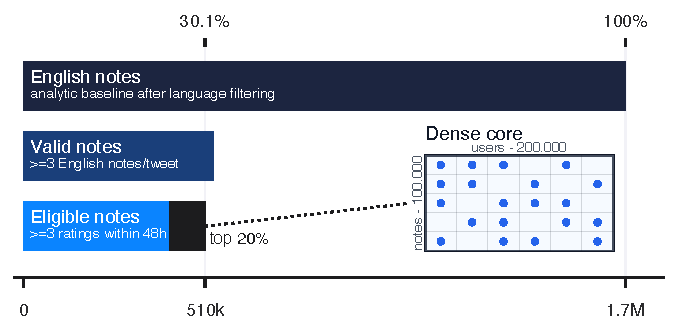
\includegraphics[width=\columnwidth]{../figures/script_figures/fig2-dataset-construction.pdf}
  \caption{Construction of the analytical sample. Starting from 1.7M English
  notes, we retain notes on tweets carrying at least three English-language
  candidate notes, and keep a note only if it drew at least three eligible
  helpful/not-helpful ratings within 48 hours of its creation, yielding 510k
  eligible notes; from these we select a 100k-note dense slice (about the top
  20\% by rating volume) and retain 200k active raters for clustering.}
  \label{fig:dataset-construction}
\end{figure}

\subsection{Recovering Constituencies}

Section~\ref{sec:cca} states behavioral recovery (P4) as a criterion; this
subsection is how we discharge it. The 200k-rater scale was selected
empirically as the best balance between coverage and diagnostic quality: as
less-active raters entered the sample, shared-note overlap thinned while a
small hyperactive core remained among the graph's most reproducible structures
\citep{nudo2026hyperactive,razuvayevskaya2025timeliness}.
Table~\ref{tab:scaleup} reports the ladder and
Appendix~\ref{app:scale-selection} the selection argument.

On that slice we build a sparse, mean-centered user-by-note matrix, where each
entry records a rater's deviation from their own average rating on a note they
scored, and embed a symmetric nearest-neighbor co-rating graph spectrally
(Appendix~\ref{app:spectral}). Constituencies are therefore recovered from
rating behavior alone, independently of any quantity X's model estimates. We
evaluate candidate values of $k$ from 2 to 7 and select the one with the
highest mean bootstrap ARI. At 200k raters that rule returns $k=3$, at ARI
0.971 against 0.593 for $k=2$, while silhouette points the other way. The two
criteria diverge because a direct $k=2$ specification must represent two
structures with only two labels: the division between the large camps and a
recurring clique of power-voters. Selecting $k=3$ makes both visible at once:
two large camps and a third cluster of 64 highly active raters, too small to be
granted constituency standing.

We therefore keep both large camps fixed and reassign only those 64, each to
whichever constituency their note-level vote profile tracks more closely
(Method B), leaving final sizes of 107,734 and 92,266 raters. This preserves the
main-camp boundary recovered at $k=3$ rather than reproducing the unstable cut
obtained by forcing two clusters. Nothing downstream turns on how the
reassignment is done: an embedding-centroid variant (Method A) sorts 29 of the
64 differently, and both partitions return the same between-camp correlation of
$-0.620$ and the same 81.4\% discriminating share
(Appendix~\ref{app:methods-ab}).

\subsection{Selection}

For each tweet, the Representative strategy selects the single note with the
highest cross-constituency score among its candidate notes
(Eq.~\eqref{eq:cca-score}). That score is defined only once both constituencies
have contributed at least three ratings (Section~\ref{sec:data-pipeline}), the
coverage rule that operationalizes P1, so notes below the bar cannot be selected
at all. A note is CCA-selected
when its bridge score exceeds 0.5, and newly rescued when it is CCA-selected but
not already shown by Community Notes.

\subsection{Validation}

Aggregation and content quality are different judgments, and we keep them
separate: CCA identifies notes that clear a cross-constituency support bar, and
an independent stage asks whether the note itself is worth showing. We use
Gemma 4 31B IT, the strongest open-weight model that runs unquantized on our
two-GPU allocation (Appendix~\ref{app:gemma-selection}), judging each
of the 13,655 notes in the frozen rescue pool independently through a
single-turn, zero-shot, rubric-based prompt. Appendix~\ref{app:gemma-runtime}
reports the full configuration and Appendix~\ref{app:gemma-prompts} the three
canonical prompts verbatim. Rubric-based LLM-as-a-judge measurement has broader
empirical precedent \citep{asirvatham2026gptmeasurement}, though none that
validates this model or this rubric (Appendix~\ref{app:llm-judge}).

The model sees only the note's own text; it does not see the tweet the note
responds to, open any cited URL, or observe the note's upstream selection
score. This is a real constraint on what the stage can certify
(Section~\ref{sec:limitations}): the judgment concerns the note as a
self-contained piece of writing, not the truth of its claim or its relevance to
the post it was attached to.

Validation begins with a content screen and ends with scoring. Stage 1 sorts
each note into one of five content categories, requiring a visible external
source pointer before a note can be classified as sourced factual information;
notes read as unsourced claims, irrelevant or spam, or hostile in tone stop
here. Opinion- or speculation-labeled notes receive a targeted second reading:
Stage 1.5 asks whether they contain a substantial sourced factual core that
remains informative once the subjective framing is set aside, and those that do
join the direct Stage 1 passes in a common Stage 2 pool. Stage 2 scores every
note in that pool for source traceability, the strength of the link between
claim and source, clarity and neutrality of language, and constructive rather
than hostile presentation, passing at 50 or higher. Throughout, a missing
source is scored as a validation failure, not as evidence that the underlying
claim is false: the rubric measures what the note visibly demonstrates about
itself, not what an independent investigation would find.

The exact model revision, prompt text, input manifest, and decoding seed are
recorded, as are all 25,804 attempt statuses, so any individual judgment can be
regenerated independently (Appendix~\ref{app:audit-trail}). One Stage 1 note
remained unresolved, which accounts for the difference between 25,734 logical
judgments and 25,733 accepted outputs.

\section{Results}
\label{sec:results}

\subsection{Rescue Pool and Visibility}

Of 44,722 representative-picked notes, Community Notes currently displays
6,832, about 15\%. Applying the CCA rule to the same universe qualifies
20,405 notes, 46\%, once every note that clears the coverage bar and the 0.5
bridge threshold is counted. The two sets are not nested: 6,750 of the
20,405 CCA-qualified notes are already shown, while 82 currently shown notes
fail the CCA threshold outright. CCA is not a strict superset of the platform's
display decision; it disagrees in both directions. Setting those 82 aside, the
13,655 CCA-qualified notes Community Notes does not display form the rescue
pool that the rest of this section evaluates
(Table~\ref{tab:rep-cn-overlap}, Figure~\ref{fig:rescue-panels}). Coverage is
rarely why the remaining picks fall short: only 71 of them never receive three
ratings from both constituencies, and across the full 100k-note slice only 185
notes of any kind go unscored for lack of coverage. The rest are scored and
simply fall short, at a median bridge score of 0.291. Most of what CCA
declines, it declines on the merits of the ratings it has.

\begin{figure}[h]
  \centering
  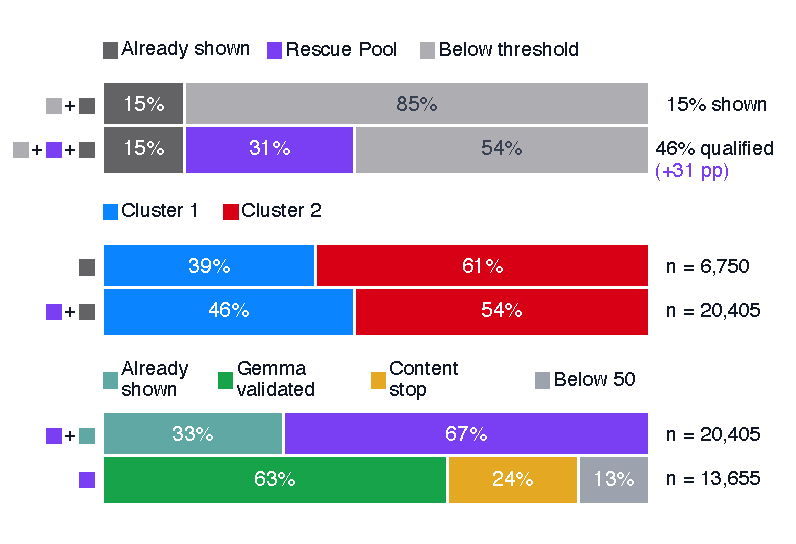
\includegraphics[width=\columnwidth]{../figures/script_figures/fig3-rescue-panels.pdf}
  \caption{Cross-constituency aggregation expands the qualified set and validates
  hidden candidates. Among 44,722 representative-picked notes, 20,405 meet the
  CCA threshold: 6,750 are already shown and 13,655 form the hidden rescue pool.
  Gemma validates 8,558 candidates; 3,279 stop at the content screen, and 1,818
  receive rescue-worthiness scores below 50.}
  \label{fig:rescue-panels}
\end{figure}

\begin{table}[t]
\centering
\small
\begin{tabular}{l r}
\toprule
\textbf{Note set} & \textbf{Count} \\
\midrule
Representative-picked note universe & 44{,}722 \\
CN shown within representative picks & 6{,}832 \\
CCA-qualified & 20{,}405 \\
\quad shown by CN & 6{,}750 \\
\quad hidden (rescue pool) & 13{,}655 \\
Below CCA threshold & 24{,}317 \\
\midrule
Rescue pool: Gemma-validated ($\geq$50) & 8{,}558 \\
Rescue pool: below score 50 & 1{,}818 \\
Rescue pool: stopped at content screen & 3{,}279 \\
\bottomrule
\end{tabular}
\caption{Representative-picked notes shown by Community Notes versus the CCA
rescue pool and its two-stage Gemma validation outcome.}
\label{tab:rep-cn-overlap}
\end{table}

\subsection{Validation Outcomes}

Stage 1 sorts the 13,655-note rescue pool by content type: 10,096 notes carry
a visible external source and are read as sourced factual information, while
1,703 read as opinion or speculation, 1,340 as irrelevant or spam, 373 as
unsourced claims, and 142 as hostile in tone, with one note left unresolved.
Stage 1.5 rechecks the 1,703 opinion-labeled notes for a sourced factual core
underneath the opinion framing and recovers 280 of them, leaving 1,423 as a
genuine content stop. The 10,096 strict passes plus the 280 recalled notes
give an expanded Stage 2 population of 10,376 notes scored for
rescue-worthiness. Of these, 8,558 clear the 50-point threshold, 62.7\% of
the original rescue pool, while 1,818 score below it and 3,279 stop at the
content screen. Only 31 of the validated notes were recovered through Stage
1.5; the other 8,527 passed Stage 1 directly.

The score distribution inside Stage 2 is not evenly spread.
Figure~\ref{fig:validation-funnel} plots both stages together: most of what
the content screen stops is opinion without a sourced core, and most of what
survives to scoring scores well above the display threshold rather than barely
over it, with 43\% of the scored population in the top 90-to-100 band.

\begin{figure}[h]
  \centering
  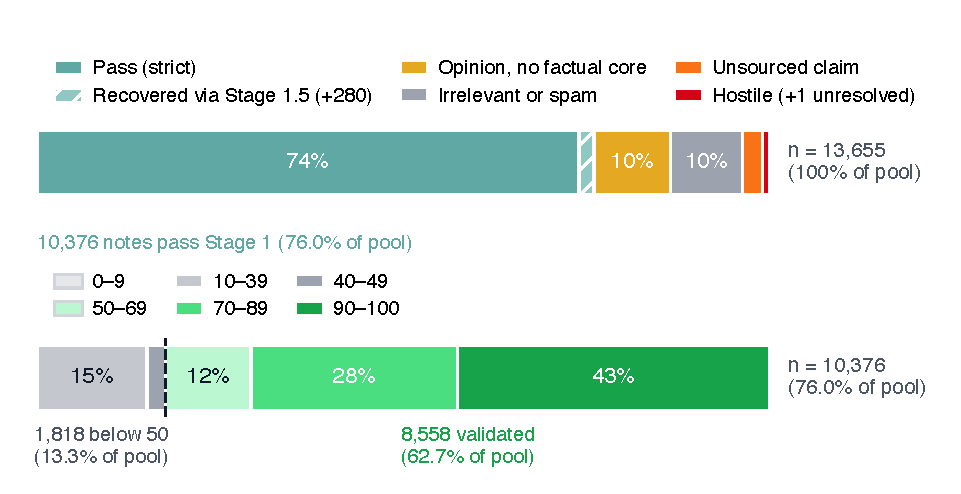
\includegraphics[width=\columnwidth]{../figures/script_figures/cn-gemma-validation-funnel.pdf}
  \caption{Two-stage Gemma validation of the 13,655-note rescue pool. The upper
  bar reports the Stage 1 content screen together with the Stage 1.5 recall,
  which recovers 280 opinion-labeled notes with a sourced factual core. The
  lower bar reports Stage 2: the 10,376 notes that pass are scored 0--100 for
  rescue-worthiness against a 50-point display threshold.}
  \label{fig:validation-funnel}
\end{figure}

\subsection{Topical Structure}

Section~\ref{sec:cca} argued from the clustering ladder alone that the two
constituencies are not simply a strict camp and a lenient one. Grouping
2,181 topically labeled notes into 13 subject areas and computing each
constituency's average approval within each gives that claim a direct test.
Figure~\ref{fig:topic-signatures} plots the result: Cluster 2 approves more
readily on 8 of the 13 topics, while Cluster 1 leads on the other five,
including Israel/Palestine content, Iranian politics, and coverage of the
Gaza hostages, so approval leadership is not fixed across the board, and the
size of the gap varies severalfold across topics
(Figure~\ref{fig:topic-signatures}). A single strictness axis would predict one
constituency leading everywhere by a roughly constant margin; what the topic
breakdown shows instead is two constituencies whose disagreement is
topic-specific, consistent with recovering distinct viewpoints rather than one
careful reader and one permissive one.

\begin{figure}[h]
  \centering
  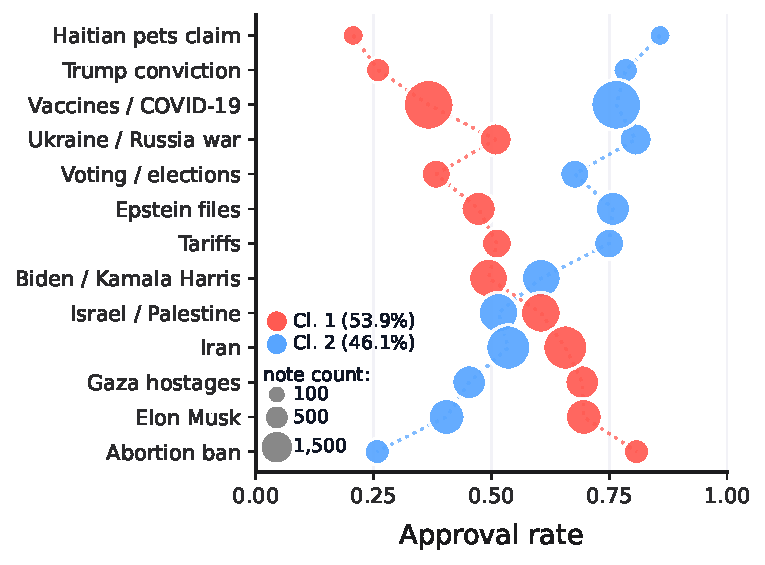
\includegraphics[width=\columnwidth]{../figures/script_figures/cn-topic-signatures.pdf}
  \caption{Average approval rate by constituency across 13 subject areas.
  Bubble size encodes note count. Approval leadership flips between
  constituencies across topics, and the size of the gap ranges from 0.090 on
  Israel/Palestine content to 0.651 on a fabricated claim about Haitians and
  pets.}
  \label{fig:topic-signatures}
\end{figure}

\subsection{Illustrative Rescue Cases}

Aggregate counts conceal two distinct ways CCA changes a display decision.
We therefore inspect six purposively selected cases: three from the 8,339
Gemma-validated CCA selections on tweets where Community Notes displays no
note, and three from the 219 validated selections where the same tweet already
has a different displayed note. The examples illustrate the rule's behavior
rather than estimate the average quality of either population.
Tables~\ref{tab:hidden-rescue-cases} and \ref{tab:better-alternatives}
reproduce them and their linked sources in full.

\urldef{\rawChickenStudyUrl}\url{https://www.fsis.usda.gov/sites/default/files/media_file/2021-02/FSCRP_Year%2B2_Final_Aug2019.pdf}
\urldef{\mutahShownWikiUrl}\url{https://en.wikipedia.org/wiki/Battle_of_Mu%27tah#:~:text=Notes%20%5E%20The%20Byzantines%20do%20not%20appear,uncertain%2C%20but%20unlikely%20to%20have%20exceeded%2010%2C000.}
\urldef{\mutahShownHistoryUrl}\url{https://islam365.io/topics/wars.html#:~:text=The%20Muslim%20army%20marched%20north%20to%20Mu'tah%2C,Muslims%20were%20greatly%20outnumbered%20(perhaps%20by%20ten%2Dto}
\urldef{\mutahCcaWikiUrl}\url{https://en.wikipedia.org/wiki/Battle_of_Mu%27tah}

\begin{table*}[t]
\centering
\footnotesize
\setlength{\tabcolsep}{3pt}
\renewcommand{\arraystretch}{1.12}
\begin{tabularx}{\textwidth}{@{}p{2.4cm}>{\raggedright\arraybackslash}Xrrr@{}}
\toprule
\textbf{Case} & \textbf{CCA-selected note (verbatim)} &
\textbf{Global} & \textbf{CCA score} & \textbf{Gemma} \\
\midrule
Raw chicken safety &
Raw chicken does not need to be washed before cooking. Washing poultry prior
to cooking it has been found to slightly increase bacterial contamination in
the kitchen. \url{https://www.cdc.gov/food-safety/foods/chicken.html}
\rawChickenStudyUrl
& 95.1\% & 0.941 & 98 \\
\addlinespace
Eisenhower and Suez &
Factual error: U.S. President Dwight D. Eisenhower insisted that Israel
withdraw from Arab territory during the 1956 Suez Crisis.
\url{https://www.presidency.ucsb.edu/documents/message-prime-minister-ben-gurion-urging-withdrawal-israeli-forces-egypt}
& 84.6\% & 0.817 & 98 \\
\addlinespace
Trump--Colorado ballot ruling &
The Supreme Court unanimously ruled Trump could not be taken off the ballot by
Colorado under Section 3 of the 14th Amendment because states do not have the
power to do so. It wasn't a matter of not ``holding him accountable'' for
January 6. \url{https://www.supremecourt.gov/opinions/23pdf/23-719_19m2.pdf}
& 92.1\% & 0.735 & 98 \\
\bottomrule
\end{tabularx}
\caption{Validated CCA selections for three tweets on which Community Notes
displays no note. Note wording and source URLs are reproduced in full; only
quotation marks and spacing are normalized for typesetting.
``Global'' is overall approval, ``CCA score'' is the geometric mean of the two
constituency-specific approval rates, and ``Gemma'' is the Stage 2
rescue-worthiness score.}
\label{tab:hidden-rescue-cases}
\end{table*}

\begin{table*}[t]
\centering
\fontsize{7.5}{8.8}\selectfont
\setlength{\tabcolsep}{3pt}
\renewcommand{\arraystretch}{1.04}
\begin{tabularx}{\textwidth}{@{}p{2.1cm}p{1.25cm}>{\raggedright\arraybackslash}Xrrr@{}}
\toprule
\textbf{Case} & \textbf{Decision} & \textbf{Note (verbatim)} &
\textbf{Global} & \textbf{CCA score} & \textbf{Gemma} \\
\midrule
Yarmouk/Mu'tah & X shown &
The Battle of Mu'tah was fought between the Byzantine Empire and the First
Islamic State. The true size of the armies is considered to be around 10,000
for the Byzantines and 3000 for the Muslims. It ended with a Byzantine
victory.
\mutahShownWikiUrl
\mutahShownHistoryUrl
& 92.2\% & 0.774 & --- \\
& CCA &
The post refers to the Battle of Yarmouk (636 AD), but reliable estimates put
Muslim forces at 15,000-40,000, not 3,000, vs. 15,000-150,000 Byzantines.
3,000 Muslims fought at the earlier Battle of Mu'tah (629 AD).
\url{https://en.wikipedia.org/wiki/Battle_of_the_Yarmuk}
\url{https://www.britannica.com/topic/Battle-of-Yarmouk-636}
\mutahCcaWikiUrl
& 91.2\% & 0.837 & 95 \\
\addlinespace
Anne Frank graphic adaptation & X shown &
Diary of a Young Girl, by Anne Frank, is part of the 8th-grade curriculum of
the Florida Department of Education.
\url{https://www.fldoe.org/core/fileparse.php/7539/urlt/pgg-8-standards.pdf}
\url{https://www.fldoe.org/core/fileparse.php/7539/urlt/elabeststandardsfinal.pdf}
& 97.8\% & 0.781 & --- \\
& CCA &
Florida removed the graphic novel adaptation of Anne Frank's diary due to
nudity deemed unsuitable for kids, but the original diary remains available.
Source:
\url{https://www.wafb.com/2023/04/10/graphic-novel-version-anne-frank-book-removed-by-florida-school/}
& 97.8\% & 0.848 & 95 \\
\addlinespace
Cardinal Burke/Vigan\`o & X shown &
Mr Vigano is a former archbishop who was excommunicated from the church in
2024 for schism.
\url{https://www.pillarcatholic.com/p/archbishop-vigano-excommunicated}
& 89.9\% & 0.783 & --- \\
& CCA &
The image shows Cardinal Raymond Burke, not Archbishop Vigan\`o. Vigan\`o was
excommunicated for schism in July 2024 and holds no Church office.
\url{https://www.vaticannews.va/en/vatican-city/news/2024-07/vigano-excommunicated-for-schism.html}
\url{https://thecatholicherald.com/article/cardinal-burke-appeals-to-pope-leo-for-restoration-of-traditional-latin-mass}
& 94.2\% & 0.871 & 95 \\
\bottomrule
\end{tabularx}
\caption{Same-tweet cases where CCA selects a stronger alternative to the note
displayed by Community Notes. Each pair contains the tweet's only displayed
note and the different, higher-scoring CCA selection. Text and URLs are
reproduced in full under the same normalization described in
Table~\ref{tab:hidden-rescue-cases}. ``Global'' is overall approval, ``CCA
score'' is the geometric mean of the two constituency-specific approval rates,
and ``Gemma'' is the Stage 2 rescue-worthiness score, reported only for the
CCA-selected notes.}
\label{tab:better-alternatives}
\end{table*}

The hidden cases show that rescue is not confined to one type of controversy:
a public-health correction, a diplomatic-history note, and a ballot-eligibility
note, each citing a primary source and each on a tweet that currently displays
nothing.

Paired comparisons make the qualitative gain more concrete. The displayed
Yarmouk note describes Mu'tah, whereas the CCA alternative identifies the
battle depicted and distinguishes the two events. In the Anne Frank case, the
alternative separates a removed graphic adaptation from the original diary
instead of treating them as one title. The final pair corrects the pictured
person's identity before explaining Vigan\`o's status. CCA raises the bridge
score in all three pairs. These purposively selected examples support a strong
comparative judgment about directness and contextual fit, not a statistical
ground-truth estimate for the full rescue pool.

\section{Discussion}

The results bear on three questions raised earlier: whether the display
decision's legitimacy claim can be made checkable, how CCA relates to other
proposed fixes for Community Notes, and what a rescue pool this size says
about crowdsourced moderation more broadly. Section~\ref{sec:learning} argued that a display decision made in a
collective name owes the affected parties a decision procedure they have
reason to accept, and that Community Notes already concedes cross-group
acceptability as its standard without being able to state it directly. The
results give that argument empirical content: P1 through P4 are no longer only
design commitments, but each attached to a number. Presence rarely has to act
as a hard veto, which is itself evidence the requirement is doing its job
quietly, since almost every note that reaches a bridge score reaches it having
been heard from both sides. Non-compensation is visible in the Yarmouk
comparison, where the CCA alternative has slightly lower raw approval than the
displayed note but stronger cross-constituency support, and so a higher bridge
score. Symmetry holds regardless of which constituency is larger or more active
on a given note. Behavioral recovery is the clustering ladder of
Section~\ref{sec:the_gap}. Because CCA is derived from stated criteria, its
design can be evaluated one commitment at a time against the evidence reported
here.

One development is already visible in the platform's own direction. In November
2025 X began piloting a final-scoring model that aggregates helpfulness through a
geometric mean of helpfulness rates across the rater-factor spectrum
\citep{xcommunitynotes2026ranking}, the soft-veto logic of CCA, adopted inside
the production pipeline but still organized along one fitted axis. The step CCA
formalizes is the obvious next one: take that geometric mean over behaviorally
recovered constituencies, each required to be present, rather than over points
on an estimated ideology line.

CCA is not the only response to the profiling critique of
Section~\ref{sec:how_cn_works}. Quality-sensitive matrix factorization
\citep{goyal2026qsmf} keeps the rater-profiling structure but weights each
rater by an estimated reliability, reaching comparable accuracy from 26--40\%
fewer ratings. The two approaches do not compete on the same axis: QSMF asks
which raters are more reliable, CCA which constituencies approve, and a
platform could run both, with reliability weighting inside each constituency
and cross-constituency consent as the gate on top. That combination is future
work, not a claim we test here.

Language-model judgment remains downstream of selection in this study: CCA
forms the rescue pool, and Gemma evaluates its contents afterward. A future
system could instead incorporate LLM judgment into CCA selection itself,
although we neither specify nor test such an integration. X's current For You
stack, which already places Grok-derived transformers inside retrieval, ranking
and policy classification \citep{xai2026algorithm}, is one concrete instance of
the broader shift toward using such models inside content-selection pipelines
rather than only after selection.

The rescue pool's size speaks to a question broader than Community Notes.
13,655 representative picks clear cross-constituency support and stay
hidden, and 8,558 of them also clear an independent content check. Some of
that gap is a rating-volume problem, the sparse participation
Section~\ref{sec:how_cn_works} describes. But the topical pattern in
Figure~\ref{fig:topic-signatures}, where the constituencies split leadership
unevenly and the size of the gap varies severalfold across topics, is not
explained by volume alone; it points to an aggregation rule that treats
uneven cross-group support as absence of consensus rather than as
consensus expressed unevenly. Crowdsourced moderation that wants to credit
genuine cross-group agreement needs a rule that can see the groups, not only
a model that infers them as a byproduct of estimating something else. Given
how much more trust a community-written note carries than a bare misleading
flag (Section~\ref{sec:learning}), which notes earn that framing is not a minor
implementation detail.

\section{Limitations}
\label{sec:limitations}

Several substantive limits accompany the design, and the empirical exercise
evaluates only one fully specified implementation.

The constitutional experience in Section~\ref{sec:learning} clarifies a
tradeoff rather than supplying a template to copy wholesale. Power-sharing can
protect one group from domination while also hardening group boundaries,
empowering actors who claim to speak for a bloc, and creating veto points that
frustrate broadly supported decisions
\citep{mcgarryoleary2009,schwartz2010,mcculloch2025}. CCA faces a platform-scale
version of the same tradeoff: treating two behavioral constituencies as the
units of consent could preserve a division that might otherwise weaken, and the
soft veto against one-sided capture could also block a note supported by a broad
but not overwhelming majority. The rule therefore applies only while
co-rating behavior supports stable, substantively sized constituencies. If that
structure disappears, forcing a group-based decision would no longer satisfy
P4, and pooled estimation becomes the more appropriate baseline.

Our final partition is a simplification, and one we impose in part. Folding
the third cluster back into the main camps is defensible on the grounds given
in Section~\ref{sec:the_gap}, but it is a decision about standing rather than a
finding about the data, and political disagreement on the platform is not
thereby shown to be binary.
Behavioral constituencies recovered from co-rating patterns need not track
any external category such as party or country; we make no claim that they
do, and a finer or differently structured partition might recover distinct
behavior our two-camp setup collapses together.

Content validation carries a different set of boundaries. Gemma judges each
note as a self-contained piece of writing: it never sees the tweet the note
responds to or opens a cited source, so a passing score certifies visible
sourcing and internal coherence, not that the source supports the claim or
that the note addresses the post. Giving a validation model both the original
tweet and access to the cited material would broaden the task to include those
two judgments, but we did not test a retrieval-enabled setup. Nor did we
compare Gemma 4 31B IT with other or larger models, which could produce
different classifications and score calibration. The run also uses one
temperature, lacks a human-rated comparison sample and inter-rater agreement
check, and fixes the 0.5 bridge and 50-point rescue-worthiness thresholds
without sensitivity sweeps. Content validation is not immune to the
manipulation risk that motivated Section~\ref{sec:how_cn_works}: an aggregation
rule that resists a hyperactive rating minority still depends on a note-quality
check that has not been stress-tested against adversarial writing
\citep{truong2025vulnerable}.

Coverage is bounded on several fronts at once. The dataset is
English-only, restricted to a 48-hour rating window, and drawn from roughly
the top 20\% of notes by rating volume, so results here describe the densest,
most active part of the platform, not its long tail. Finally, the minimum-coverage
requirement that discharges P1 leaves thinly rated notes unscored rather than
risk a decision on too little evidence. We set that presence floor at three
ratings per constituency but did not test alternatives such as four, five, or
higher. Raising it could reduce sampling noise within each constituency while
also leaving more notes unscored. Broader participation could make some of the
excluded notes scorable, but it would not change the verdict on the tens of
thousands that already have sufficient coverage and fall below the bridge
threshold. The reported configuration should be read as a fully documented
implementation, not as evidence that these settings are optimal.

\section{Conclusion}

Community Notes already commits to cross-group acceptability as its display
standard; it just cannot state that standard directly, because its rating model
never forms the constituencies the standard is about. This paper recovers those
constituencies from rating behavior and makes the standard explicit: a geometric
mean of within-constituency approval, gated by a coverage requirement that keeps
any single constituency from being counted without being heard. Applied to the
platform's own representative picks, the rule surfaces 13,655 notes that clear
cross-constituency support and remain hidden, of which 8,558 also pass an
independent content check. Neither number is the platform's final answer on any
of these notes; both are evidence that a meaningful share of what disappears
into Needs More Ratings disappears for a reason the aggregation rule creates. The broader claim is not specific to Community Notes: any system
that decides visibility, in a collective name, over a durably divided
audience faces the same choice we describe in Section~\ref{sec:learning},
between compressing disagreement into one pooled score and preserving its
structure long enough for every relevant part of the audience to be heard
from. We think cross-constituency aggregation should be treated as an
alternative design feature of crowdsourced moderation systems.

\section*{Acknowledgments}

The authors acknowledge support by the local computing resources through the
core facility SCCKN (\url{https://scc.uni-konstanz.de}).

\bibliographystyle{plainnat}
\bibliography{references}

\onecolumn
\appendix
\section{Pipeline and Constituency Recovery}
\label{app:pipeline}

This appendix holds the operational detail behind
Section~\ref{sec:approach}. Every threshold and variant reported here is also
implemented in the accompanying repository.

\subsection{Filter thresholds and the two three-rater floors}
\label{app:filters}

A floor of three applies at both the candidate-note and the rating stage, but
for distinct operational reasons: the first guarantees a genuine multi-note
choice set, while the second follows the same minimum-coverage logic that X
applies before cross-viewpoint evidence can affect a note's status. The rating
floor establishes minimal observed participation rather than claiming a
reliable estimate of approval \citep{xcommunitynotes2026ranking}.

\subsection{Selecting the 200k rater scale}
\label{app:scale-selection}

The scale was chosen by testing rather than assumed. The tests encountered the
same participation imbalance identified for Community Notes in
Section~\ref{sec:the_gap}: as progressively less-active raters entered the
sample, shared-note overlap thinned, while a small hyperactive core remained
among the graph's most reproducible structures. We selected 200k as the best
balance between coverage and diagnostic quality. 210k reproduced the same
two-camp structure somewhat more weakly, while larger configurations
introduced additional activity-driven outliers or collapsed into a
power-voter-versus-rest split.

\subsection{Spectral embedding and outlier handling}
\label{app:spectral}

A symmetric 15-nearest-neighbor graph over the mean-centered user-by-note
matrix defines co-rating similarity, and a spectral embedding, computed with
algebraic multigrid to keep the procedure tractable at this scale, places each
rater in a low-dimensional space shaped by whom they tend to agree with.
Candidate values of $k$ from 2 to 7 are evaluated by silhouette score and by
stability under repeated resampling. Where a direct $k=2$ specification is
forced, it sometimes recovers the balanced camp split across resamples and
sometimes uses one label to isolate the small, highly active group; the same
high-activity pattern reappears at neighboring scales. Clusters smaller than
$\max(1\%$ of raters$, 500)$ are treated as outliers rather than granted
constituency standing.

\subsection{Reassignment: Method A versus Method B}
\label{app:methods-ab}

Method B is not another $k=2$ spectral fit. It begins from the more stable
$k=3$ partition, keeps the membership of both large camps fixed, and
classifies only the 64 outliers, correlating each outlier's note-level vote
profile against the two main constituencies' aggregate profiles. Method A, an
embedding-centroid variant, sorts the same 64 raters by distance in the
spectral embedding instead. The two rules disagree about 29 of the 64, who
together cast 0.07\% of the ratings in the slice, and the resulting partitions
return the same between-camp correlation of $-0.620$ and the same 81.4\%
discriminating share. Method B is the canonical partition used throughout the
paper; the original spectral label survives only as a diagnostic column.

\section{Gemma Validation Runtime}
\label{app:gemma-runtime}

Table~\ref{tab:gemma-runtime} records the canonical configuration of the
validation run.

\begin{table}[ht]
\centering
\small
\begin{tabularx}{\textwidth}{@{}p{2.7cm}>{\raggedright\arraybackslash}X@{}}
\toprule
\textbf{Component} & \textbf{Canonical configuration} \\
\midrule
Model & \texttt{google/gemma-4-31B-it}; 30.7B dense parameters; revision
\texttt{518276fb130dc81caf9a4f772e65e63ef2526493}; instruction-tuned thinking
variant; BF16; no quantization. \\
Hardware & Two NVIDIA L40S GPUs, 46,068 MiB reported memory each; tensor
parallelism 2. SCCKN AMD EPYC host with eight allocated CPU slots; SGE request
of 64 GB \texttt{h\_vmem} per slot and approximately 52 GB observed peak
\texttt{maxvmem} (host memory, not GPU memory). \\
Serving & Locally hosted vLLM 0.25.0 inference server, bound to
\texttt{127.0.0.1} and accessed through its \texttt{/v1} HTTP endpoint; CUDA
13.2; PyTorch 2.11.0+cu130; Transformers 5.13.1; asynchronous scheduling;
prefix caching; 64 concurrent requests and maximum sequences; 32,768 maximum
batched tokens; 90\% GPU-memory-utilization target. \\
Decoding & Thinking enabled with the Gemma 4 reasoning parser; temperature
0.2; 8,192-token context cap; 4,096-token completion cap; deterministic seed
from SHA-256 of base seed 42, stage, note ID, and attempt number. \\
Prompt contract & One note per independent user prompt; no system prompt,
few-shot examples, guided generation, tweet context, URL fetching, retrieval,
embeddings, vector store, upstream selection score, or Gabriel label. The model
receives only the note text and stage-specific instructions. \\
Validation and retry & Unconstrained generation followed by strict JSON output
validation; maximum three attempts. Every attempt retains its seed and status;
returned outputs are stored with the parsed result, reasoning, and token counts,
while response failures retain error metadata. \\
Run scale & 25,734 logical judgments across Stages 1, 1.5, and 2; 25,733
accepted judgments from 25,804 attempts; 99.75\% valid on the first attempt;
32,113,128 prompt-and-completion tokens; 12h 28m summed active-phase time and
15h 51m from first to final output, including inter-stage gaps. \\
\bottomrule
\end{tabularx}
\caption{Canonical Gemma validation configuration. Model-family properties and
the Arena snapshot come from the official model materials and Arena
leaderboard \citep{arena2026leaderboard,google2026gemma4,google2026gemma4card};
run-specific values come from the frozen manifests, SCCKN scheduler records,
worker configuration, and per-attempt audit logs; vLLM is described by
\citet{kwon2023vllm}.}
\label{tab:gemma-runtime}
\end{table}

\subsection{Model selection and serving constraints}
\label{app:gemma-selection}

Gemma 4 31B IT was the strongest feasible open-weight model for this role. In
the April 2, 2026 Arena snapshot, its thinking variant scored 1,452 and ranked
third among open models, while its 30.7-billion-parameter dense BF16 weights
could run without quantization on our two-GPU allocation
\citep{arena2026leaderboard,google2026gemma4}.

\subsection{Rubric-based LLM-as-a-judge precedent}
\label{app:llm-judge}

Across 1,141 human-labeled binary classification tasks, GABRIEL reports a
median accuracy of 0.85 for GPT-5 and finds measurements generally robust to
semantically equivalent prompt variants \citep{asirvatham2026gptmeasurement}.
This benchmark supports the feasibility of large-scale qualitative judgment,
but it does not validate Gemma or the task-specific rubric used here.

\subsection{Audit trail and output validation}
\label{app:audit-trail}

Every returned response is stored with its parsed result, reasoning, and token
counts; the 71 response errors retain their seed and error metadata but
contain no output fields because no model response was returned. Generation is
not schema-constrained. Responses are parsed and checked against a strict
contract afterward: an exact key set, a label drawn from the fixed list or an
integer score in range, and a reason under forty words, with at most three
attempts before a judgment is left unresolved. This audit trail allows any
individual judgment to be regenerated independently while preserving the
distinction between model output and post-generation validation.

\section{Canonical Gemma Validation Prompts}
\label{app:gemma-prompts}

The prompts below are included directly from the tracked artifacts used by the
canonical run. At inference time, \verb|{note_text}| was replaced by the
text of one Community Note; no system prompt or additional contextual message
was supplied. The manifest hashes were computed over the template text before
the tracked artifact's terminal newline:
\begin{itemize}[nosep,leftmargin=1.7cm]
  \item[Stage 1:] \texttt{fbbd4bd93fb419ad66cce097bb18a8705fd331f38ec1a9bf433aa783281023d2}
  \item[Stage 1.5:] \texttt{26114bb8632357166cf4cee9a4f0ce356ed1e9e527477d56c842e53415bc930f}
  \item[Stage 2:] \texttt{8c98c54b9c413ee70c161f40ec8e89f0b19ac6420b2bfe669e7ee1f9b136c644}
\end{itemize}

\subsection{Stage 1: Content Classification}
\VerbatimInput[fontsize=\scriptsize]{../data/llm_validation/runs/gemma-4-31b-it-scckn-v1/stage1_prompt.txt}

\subsection{Stage 1.5: Sourced-Factual-Core Recall}
\VerbatimInput[fontsize=\scriptsize]{../data/llm_validation/runs/gemma-4-31b-it-scckn-stage1-5-opinion-v1/stage1_5_prompt.txt}

\subsection{Stage 2: Rescue-Worthiness Scoring}
\VerbatimInput[fontsize=\scriptsize]{../data/llm_validation/runs/gemma-4-31b-it-scckn-stage2-expanded-v1/stage2_prompt.txt}

\end{document}
